\documentclass{beamer} %[aspectratio=1610]

\usetheme{Darmstadt}
\usefonttheme[onlylarge]{structurebold}
\setbeamerfont*{frametitle}{size=\normalsize,series=\bfseries}
\setbeamertemplate{navigation symbols}{}

% Standard packages

\usepackage[english]{babel}
\usepackage[latin1]{inputenc}
\usepackage{times}
\usepackage[T1]{fontenc}
\usepackage{float}
\usepackage{graphicx}
\usepackage{subcaption}
\usepackage{ifthen}
\usepackage{minted}
\usepackage{verbatim}
%\usepackage{multimedia}
\usepackage[]{algorithm2e}

% Setup TikZ
\usepackage{tikz}
\usetikzlibrary{arrows}
\tikzstyle{block}=[draw opacity=0.7,line width=1.4cm]


% Author, Title, etc.
\title[Show me your properties! The potential of property-based testing in Agent-Based Simulation] 
{%
  Show me your properties! \\ \tiny{The potential of property-based testing in Agent-Based Simulation}
}

\author[Thaler]
{
  Jonathan~Thaler
}

\institute[University of Nottingham, Nottingham, United Kingdom]
{
  University of Nottingham, Nottingham, United Kingdom
}

\date[SummerSim'19, July 22-24, Berlin, Germany]
{SummerSim'19, July 22-24, Berlin, Germany}

% The main document

\begin{document}

\begin{frame}
  \titlepage
\end{frame}

\section{Introduction}
\begin{frame}{Code testing in ABS?}
\begin{itemize}
	\item Very neglected but important!
	\item One paper \footnote{Collier, N., and Ozik, J. Test-driven agent-based simulation development. In 2013 Winter Simulations Conference (WSC) (Dec. 2013),pp. 1551 - 1559.} focusing on TDD with unit testing
  	\item Unit testing not very suitable for ABS
  	\item How deal with ABS stochastic nature?
\end{itemize}

\begin{block}{Solution}
Stochastic ABS + random property-based testing = $\heartsuit \heartsuit \heartsuit$
\end{block}
\end{frame}

\section{Property-Based Testing}
\begin{frame}{Property-Based Testing}
  \begin{itemize}
    \item Express specifications directly in code
    \item \textit{QuickCheck} library generates random test cases
    \item Developer can express expected coverage
    \item Integrate into discovery and hypotheses process
  \end{itemize}
\end{frame}

\begin{frame}[fragile]{QuickCheck}
\begin{block}{List Properties}
\begin{minted}[fontsize=\footnotesize]{haskell}
-- the reverse of a reversed list is the original list
reverse_reverse xs = reverse (reverse xs) == xs

-- concatenation operator (++) is associative
append_associative xs ys zs 
  = (xs ++ ys) ++ zs == xs ++ (ys ++ zs)

-- reverse is distributive over concatenation (++)
reverse_distributive xs ys 
  = reverse (xs ++ ys) == reverse xs ++ reverse ys
\end{minted}
\end{block}
\end{frame}

\begin{frame}[fragile]{QuickCheck cont'd}
\begin{block}{Running the tests...}
\begin{footnotesize}
\begin{verbatim}
+++ OK, passed 100 tests.
+++ OK, passed 100 tests.
*** Failed! Falsifiable (after 3 tests and 1 shrink):     
[1]
[0]
\end{verbatim}
\end{footnotesize}
\end{block}
\end{frame}

\begin{frame}[fragile]{QuickCheck cont'd}
\begin{block}{Labeling}
\begin{minted}[fontsize=\footnotesize]{haskell}
reverse_reverse_label xs  
  = label ("length of list is " ++ show (length xs)) 
          (reverse (reverse xs) == xs)
\end{minted}
\end{block}

\begin{block}{Running the tests...}
\begin{footnotesize}
\begin{verbatim}
+++ OK, passed 100 tests:
 5% length of list is 27
 5% length of list is 0
 4% length of list is 19
 ...
\end{verbatim}
\end{footnotesize}
\end{block}
\end{frame}

\begin{frame}[fragile]{QuickCheck cont'd}
\begin{block}{Coverage}
\begin{minted}[fontsize=\footnotesize]{haskell}
reverse_reverse_cover xs  = checkCoverage 
  cover 15 (length xs >= 50) "length of list at least 50"
  (reverse (reverse xs) == xs)
\end{minted}
\end{block}

\begin{block}{Running the tests...}
\begin{footnotesize}
\begin{verbatim}
+++ OK, passed 12800 tests 
    (15.445% length of list at least 50).
\end{verbatim}
\end{footnotesize}
\end{block}
\end{frame}

\section{Property-Based Testing in ABS}
\begin{frame}{Property-Based Testing in ABS}
\begin{block}{Randomised Property-Based Testing}
Matches the constructive and exploratory nature of ABS
\end{block}

  \begin{itemize}
    \item Exploratory models: hypothesis tests about dynamics
    \item Explanatory models: validate against formal specification
    \item Test simulation and model invariants
    \item Test agent specification
  \end{itemize}
\end{frame}

\begin{frame}{Property-Based Testing in ABS}
\begin{block}{Randomised Property-Based Testing}
Matches the constructive and exploratory nature of ABS
\end{block}

  \begin{itemize}
    \item Exploratory models: hypothesis tests about dynamics
    \item Explanatory models: validate against formal specification
    \item Test simulation and model invariants
    \item \textbf{Test agent specification}
  \end{itemize}
\end{frame}

\begin{frame}{Test agent specification}
\begin{block}{Code / Implementation Testing}
Follow formal model specification or informal description
\end{block}

\begin{block}{}
  \begin{itemize}
  	\item Express invariants of output given random inputs
  	\item Probabilities of transitions and timeouts use \texttt{cover}
    \item Event-driven ABS: relate input events to output events 
    \item Time-driven ABS: specify output stream
  \end{itemize}
\end{block}
\end{frame}

\begin{frame}{Test agent specification}
\begin{block}{Code / Implementation Testing}
Follow formal model specification or informal description
\end{block}

\begin{block}{}
  \begin{itemize}
  	\item Express invariants of output given random inputs
  	\item Probabilities of transitions and timeouts use \texttt{coverage}
    \item Event-driven ABS: relate input events to output events 
    \item \textbf{Time-driven ABS: specify output stream}
  \end{itemize}
\end{block}
\end{frame}

\begin{frame}{Example: Agent-Based SIR Model}
\begin{center}

\includegraphics[width=0.7\textwidth]{./fig/SIR_transitions.png}
\end{center}
  \begin{itemize}
    \item Population size $N = 1,000$
 	\item Contact rate $\beta = 5$
 	\item Infection probability $\gamma = 0.05$
 	\item Illness duration $\delta = 15$
 	\item 1 initially infected agent
  \end{itemize}
\end{frame}

\begin{frame}{Dynamics of Agent-Based SIR Model}
\begin{center}
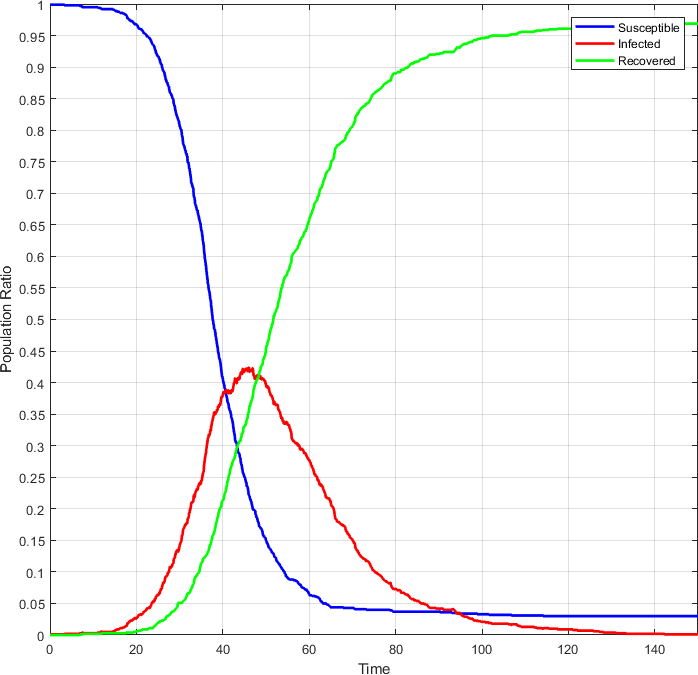
\includegraphics[width=0.7\textwidth]{./fig/SIR_Yampa_dt001.png}
\end{center}
\end{frame}

\begin{frame}[fragile]{Susceptible Agent Specification}
\begin{block}{}
\begin{minted}[fontsize=\footnotesize]{haskell}
susceptibleAgent :: SF [SIRState] SIRState

data SIRState = Susceptible | Infected | Recovered
\end{minted}
\end{block}

\begin{center}
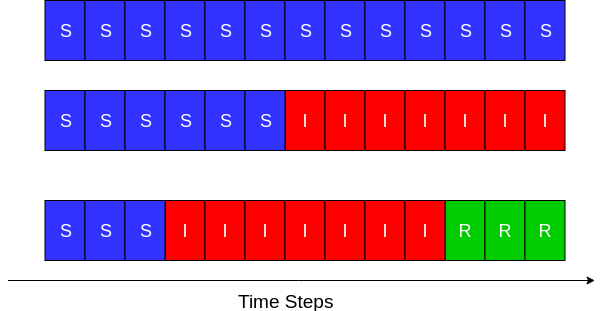
\includegraphics[width=0.9\textwidth]{./fig/property_susceptible_output.png}
\end{center}
\end{frame}

\begin{frame}[fragile]{Susceptible invariants}
\begin{minted}[fontsize=\tiny]{haskell}
susceptibleInv :: [SIRState] -- ^ output stream of the susceptible agent 
               -> Bool       -- ^ population contains an infected agent
               -> Bool       -- ^ True in case the invariant holds
susceptibleInv aos infInPop
    -- Susceptible became Infected and then Recovered
    | isJust recIdxMay 
      = infIdx < recIdx &&  -- agent has to become infected before recovering
        all (==Susceptible) (take infIdx aos) && 
        all (==Infected)    (take (recIdx - infIdx) (drop infIdx aos)) && 
        all (==Recovered)   (drop recIdx aos) &&
        infInPop  -- can only happen if there are infected in the population

    -- Susceptible became Infected
    | isJust infIdxMay 
      = all (==Susceptible) (take infIdx aos) &&
        all (==Infected)    (drop infIdx aos) &&
        infInPop -- can only happen if there are infected in the population

    -- Susceptible stayed Susceptible
    | otherwise = all (==Susceptible) aos
  where
    infIdxMay = elemIndex Infected aos
    recIdxMay = elemIndex Recovered aos
    infIdx    = fromJust infIdxMay
    recIdx    = fromJust recIdxMay
\end{minted}
\end{frame}

\begin{frame}[fragile]{Susceptible property test}
\begin{minted}[fontsize=\tiny]{haskell}
prop_susceptible :: Positive Double -- ^ contact rate
                 -> Probability     -- ^ infectivity within (0,1)
                 -> Positive Double -- ^ illness duration
                 -> TimeRange       -- ^ simulation duration
                 -> [SIRState]      -- ^ population
                 -> Property
prop_susceptible
      (Positive beta) (P gamma) (Positive delta) (T t) as = property (do  
    -- check if population contains an infected agent
    let infInPop = Infected `elem` as
    aos <- genSusceptible beta gamma delta as t
    return 
        -- label all test cases
        label (labelTestCase aos) 
        -- check invariants on output stream
        (property (susceptibleInv aos infInPop))
  where
    labelTestCase :: [SIRState] -> String
    labelTestCase aos
      | Recovered `elem` aos  = "Susceptible -> Infected -> Recovered"
      | Infected  `elem` aos  = "Susceptible -> Infected"
      | otherwise             = "Susceptible"
\end{minted}
\end{frame}

\begin{frame}[fragile]{Checking the property}
\begin{block}{Running 10,000 test cases}
\begin{footnotesize}
\begin{verbatim}
> let args = stdArgs { maxSuccess = 10000 }
> quickCheckWith args prop_susceptible

> +++ OK, passed 10000 tests:
   55.78% Susceptible -> Infected -> Recovered
   37.19% Susceptible -> Infected
    7.03% Susceptible
\end{verbatim}
\end{footnotesize}
\end{block}
\end{frame}

\section{Conclusions}
\begin{frame}{Conclusion}
	\begin{itemize}
		\item Property-Based Testing + ABS match naturally.
		\item Sufficient coverage is main difficulty.
		\item \textit{SmallCheck} enumerates test cases deterministically.
	\end{itemize}
	
\begin{block}{}
Hopefully code testing will become more common in ABS.
\end{block}
\end{frame}

\begin{frame}{}
  \begin{center}
  Thank You!
  \end{center}
\end{frame}

\bibliographystyle{acm}
\bibliography{../../writing/references/phdReferences.bib}

\end{document}